\chapter{Návrh funkcionality}
	Ďalej opíšeme ako sme navrhli naše riešenie. TODO
	
	\section{Prerekvizity}
	
		Aby naše riešenie fungovalo, budeme potrebovať server, ktorý bude slúžiť na hostovanie našej služby, databázu, ktorá bude ukladať užívateľove dáta a cloudové úložisko, ktoré bude zabezpečovať prácu so súbormi. Cloud musí poskytovať rozhranie pomocou ktorého vieme nahrávať a sťahovať dáta a taktiež musí byť schopné autorizovať rôznych užívateľov pre prístup k dátam iných užívateľov, aby sme boli schopný zdieľať súbory s inými používateľmi. 
		
	\section{Predpríprava}
		
		Keď sa používateľ rozhodne pužívať našu službu musí sa nejakým spôsobom identifikovať a autentifikovať. K tomuto poslúži nejaká forma registrácie pri ktorej si užívateľ zvolí svoje univerzálne heslo pomocou ktorého bude autorizovať akcie ako nahrávanie, sťahovanie, zdieľanie a zrušenie zdieľania dát. Následne v užívateľovom prehliadači vygenerujeme verejný a privátny kľúč, ktorý symetricky zašifrujeme pomocou už zvoleného univerzálneho hesla. Verejný aj zašifrovaný privátny kľúč uložíme na servri kde prístup k verejným kľúčom budú mať všetci používatelia no k privátnym len jeho vlastníci. Tým že privátny kľúč je zašifrovaný server nemá žiadnu informáciu o privátnom kľúči a teda schéma ostane bezpečná.
	
	\section{Nahrávanie dát}
	
		Užívateľ si v prehliadači vygeneruje, pomocou dostatočne náhodného generátoru, náhodné heslo ktorým zašifruje súbor a vypýta si od servru svoj verejný kľúč ktorým heslo zašifruje. V taktomto tvare ho môže poslať na server spolu s identifikátorom súboru. Keďže heslo je zašifrované a server nemá informáciu o privátnom kľúči užívateľove dáta by mali byť stále v bezpečí. Následne už len stačí zašifrovaný súbor nahrať na cloudové úložisko.
		
	\section{Sťahovanie dát}
	
		
	
	\section{Zdieľanie}
	
		
	\section{Zrušenie zdieľania}
	
	
	
		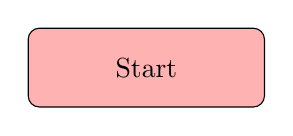
\begin{tikzpicture}
			
			\tikzstyle{startstop} = [rectangle, rounded corners, minimum width=3cm, minimum height=1cm,text centered, draw=black, fill=red!30]
			\tikzstyle{io} = [trapezium, trapezium left angle=70, trapezium right angle=110, minimum width=3cm, minimum height=1cm, text centered, draw=black, fill=blue!30]
			\tikzstyle{process} = [rectangle, minimum width=3cm, minimum height=1cm, text centered, draw=black, fill=orange!30]
			\tikzstyle{decision} = [diamond, minimum width=3cm, minimum height=1cm, text centered, draw=black, fill=green!30]
			\tikzstyle{arrow} = [thick,->,>=stealth]
			
			\node (start) [startstop] {Start};
			
		\end{tikzpicture}